\subsection{Hardware Compatible}

\subsubsection{Reducing the Input Dimension}

The size of input is determined by the dimension of inputs (originally \(16 \times 16\)) and the depth of each pixel (8-bit in the previous design).
A search is done by trying different pair of input dimension and depth and calculating the prediction accuracy using linear regression model, which is actually a lower bound we can achieve.
The result is as \autoref{fig:mnist-shrink}.

It is shown that

When the input size is shrunk to \(8 \times 8\), the misclassifications rate is 15.96\%, which is slightly worse than our target (over 85\% in accuracy).
However, this is a desirable configuration, which means we can fit an input in precisely 8 bytes.
Thus I believe it is worth sacrificing some accuracy here and getting it back using a more aggressive model.

\begin{figure}[ht!]
    \centering
    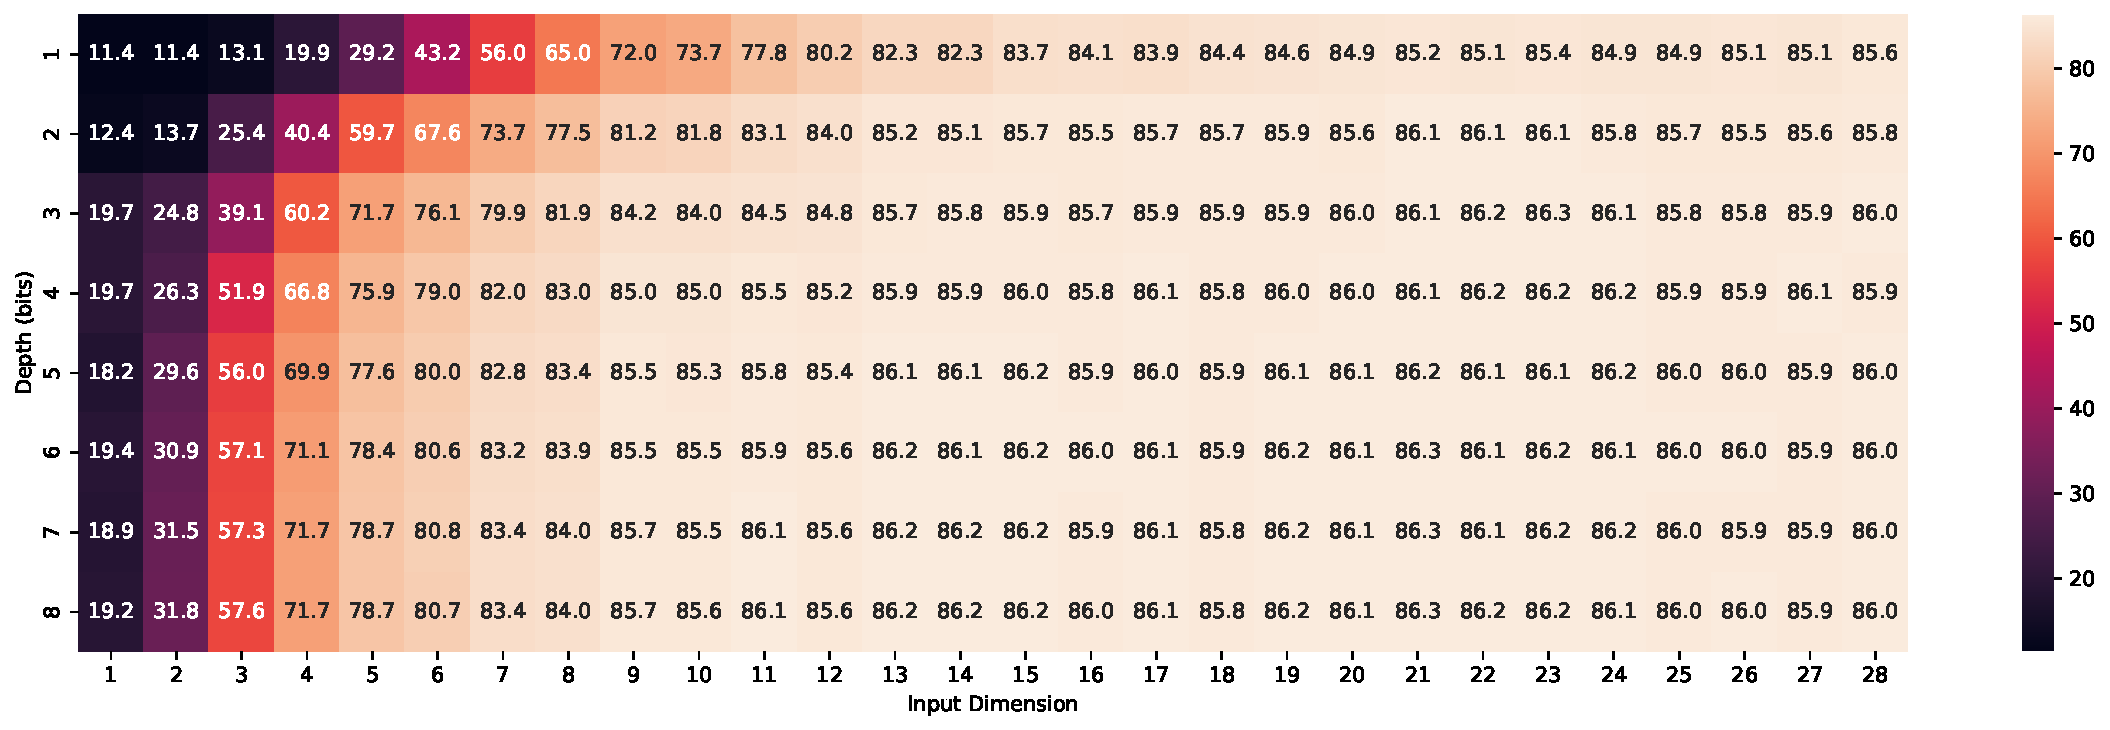
\includegraphics[width=\textwidth]{images/mnist-shrink.pdf}
    \caption{Accuracy of prediction using floating point numbers under different input size}
    \label{fig:mnist-shrink}
\end{figure}

\subsubsection{Improve Prediction Accuracy}

The accuracy is improve by using a more complex model, which includes a ReLU activated input layer (\(64 \times 16\)), which is unbiased, and a biased output layer (\(16\times 10\)).
Using ReLU with an unbiased input layer, we can refrain from floating point calculation while keep the linear property.

\[
    \mathbf{O} = \operatorname{ReLU}(\mathbf{I} \cdot \mathbf{W_1}) \cdot \mathbf{W_2} + \mathbf{b}
\]

To get a better training result, we add a Softmax layer after the model and use train towards minimized cross entropy loss.
This layer can be removed when predicting on FPGA, which will not affect the final result.


\subsubsection{Evaluation}

The design latency is 200699 cycles.

It took 4.54 ms to generate the prediction while the CPU used 169.64 ms, which means the FPGA solution achieves a 37.36x speedup against the CPU solution.
The prediction accuracy is 88.18\% on both FPGA and CPU.



\subsection{Enhancing a Single AXI Transfer}

In order to accomodate more data in a single AXI transfer\footnote{
    \href{https://developer.arm.com/documentation/ihi0051/a/Introduction/About-the-AXI4-Stream-protocol/Stream-terms}{Stream terms}
}, we need to increase the \texttt{TDATA} width.

The width in the default design is 64 bits, which took 32 cycles to transfer a single input of 256 bytes.
By widening the \texttt{TDATA} width to 256 bits, it takes only 8 cycles to transfer the 256 bytes (\autoref{tab:tdata}).

\begin{table}[ht!]
    \centering
    \caption{\texttt{LOAD\_INPUT} latency under different \texttt{TDATA} width}
    \label{tab:tdata}
    \begin{tabular}{cccccccc}
        \toprule
        \texttt{TDATA} width (bits) & Latency (cycles) & Iteration Latency & Initiation Interval (achieved) & Trip Count & Pipelined \\
        \midrule
        64                          & 4096             & 32                & 32                             & 128        & yes       \\
        128                         & 2048             & 16                & 16                             & 128        & yes       \\
        256                         & 1024             & 8                 & 8                              & 128        & yes       \\
        \bottomrule
    \end{tabular}
\end{table}


The overall latency of our design is 159646 cycles.
Its utilization is as \autoref{tab:w256}.

\begin{table}[ht!]
    \centering
    \caption{Utilization Report with 256-bit AXI Stream}\label{tab:w256}
    \begin{tabular}{cccccc}
        \toprule
        Name             & BRAM\_18K & DSP & FF     & LUT   & URAM \\
        \midrule
        DSP              & -         & 192 & -      & -     & -    \\
        Expression       & -         & -   & 0      & 4703  & -    \\
        FIFO             & -         & -   & -      & -     & -    \\
        Instance         & 0         & 0   & 36     & 1352  & -    \\
        Memory           & 202       & -   & 32     & 3     & -    \\
        Multiplexer      & -         & -   & -      & 3577  & -    \\
        Register         & -         & -   & 6552   & 128   & -    \\
        \midrule
        Total            & 202       & 192 & 6620   & 9763  & 0    \\
        \midrule
        Available        & 280       & 220 & 106400 & 53200 & 0    \\
        \midrule
        Utilization (\%) & 72        & 87  & 6      & 18    & 0    \\
        \bottomrule
    \end{tabular}
\end{table}

Since we modified the AXI data width, the data width of DMA IP needs to be fixed manually as \autoref{fig:adjust-axi-data-width}.

The evaluation shows that FPGA took 3.85 ms to produce the result, while CPU took 169.33 ms as well.
That is a 44x speedup which is better but not that better as we expected.
It is because the maximum AXI data width of Zynq 7000 processor is 64 bit, which limited the bandwidth.

The accuracy is still 88.18\%.

\begin{figure}[ht!]
    \centering
    \caption{Adjust AXI data width by re-customizing AXI-DMA IP}
    \label{fig:adjust-axi-data-width}
    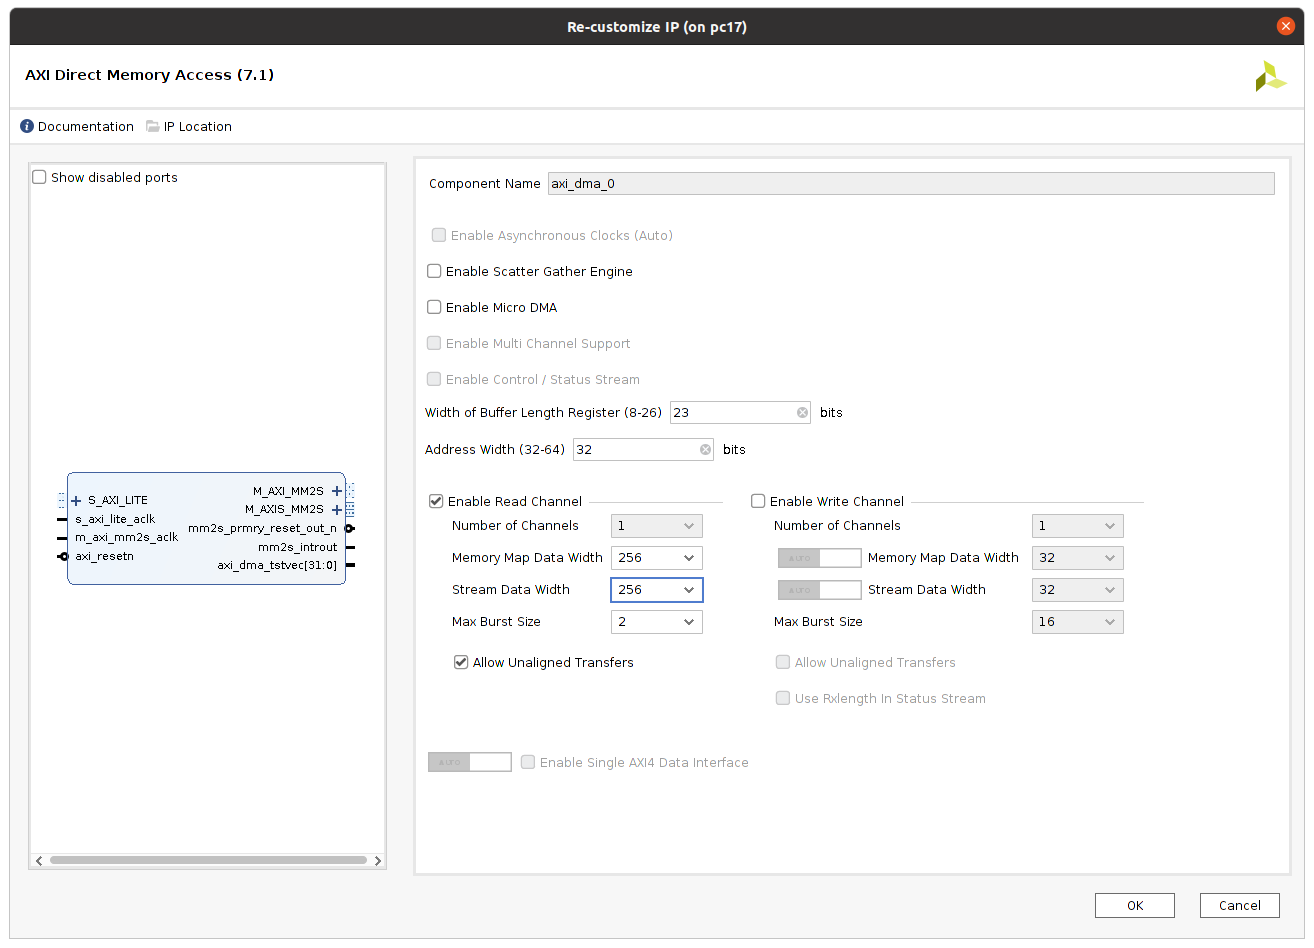
\includegraphics[scale=0.32]{images/adjust-axi-data-width.png}
\end{figure}


